%!TEX encoding = UTF-8 Unicode
% -*- coding: UTF-8; -*-
% vim: set fenc-utf-8

\chapter{Diagrammes de classe de conception}
\label{s:classe_conception}

Ce chapitre présente les différents diagrammes de classe de conception de \textit{VisualLigue}.

\section{Couche domaine}
\label{couche_domaine}

La figure \ref{fig:domaine_classe} présente le diagramme de classe de la couche applicative (domaine).
La classe \textit{Controller} est ce qui permet à la vue d'intéragir avec le domaine.
Cette classe gère les différents objets du domaines, l'éditions des stratégies ainsi que le visionnement de celles-ci.
Tout objet qui peut être placé sur le terrain est un \textit{GameObject}.
Trois classes héritent de \textit{GameObject}, soit \textit{Player}, \textit{Obstacle} et \textit{Projectile}.
Les joueurs sont maintenus dans la classe \textit{PlayerPool}, qui peut être sauvegardée.
Cela permet à l'entraîneur de réutiliser ses joueurs d'une stratégie à l'autre.
Un objet \textit{Sport} regroupe un terrain ainsi qu'une liste de rôles pour les joueurs.
Les sports sont maintenus dans la classe \textit{SportPool}, qui peut être sauvegardée, ce qui permet de réutiliser les sports créés pour différentes stratégies.
La classe \textit{Frame} représente une image du terrain avec tous les \textit{GameObject} présents à un moment précis.
La classe \textit{Strategy} regroupe tous les frames d'une stratégie et les associe à un sport.
Elle permet le visionnement ainsi que l'édition d'une stratégie.

Sous la couche domaine se trouve la couche \textit{Utility}, qui contient certaines classes et méthodes utilitaires qui sont utilisées par les classes du domaine.
Dans cette couche, on retrouve la classe Vector, qui peut représenter un vecteur 2D ou un point.
Cette couche comporte aussi le package serialization, qui contient l'interface permettant la sauvegarde et le chargement des données de l'application.
Pour éviter de surcharger le diagramme, les accesseurs et les constructeurs sans paramètre n'ont pas été représentés, bien que ces méthodes soient implémentés.

\begin{figure}[htpb]
    \centering
    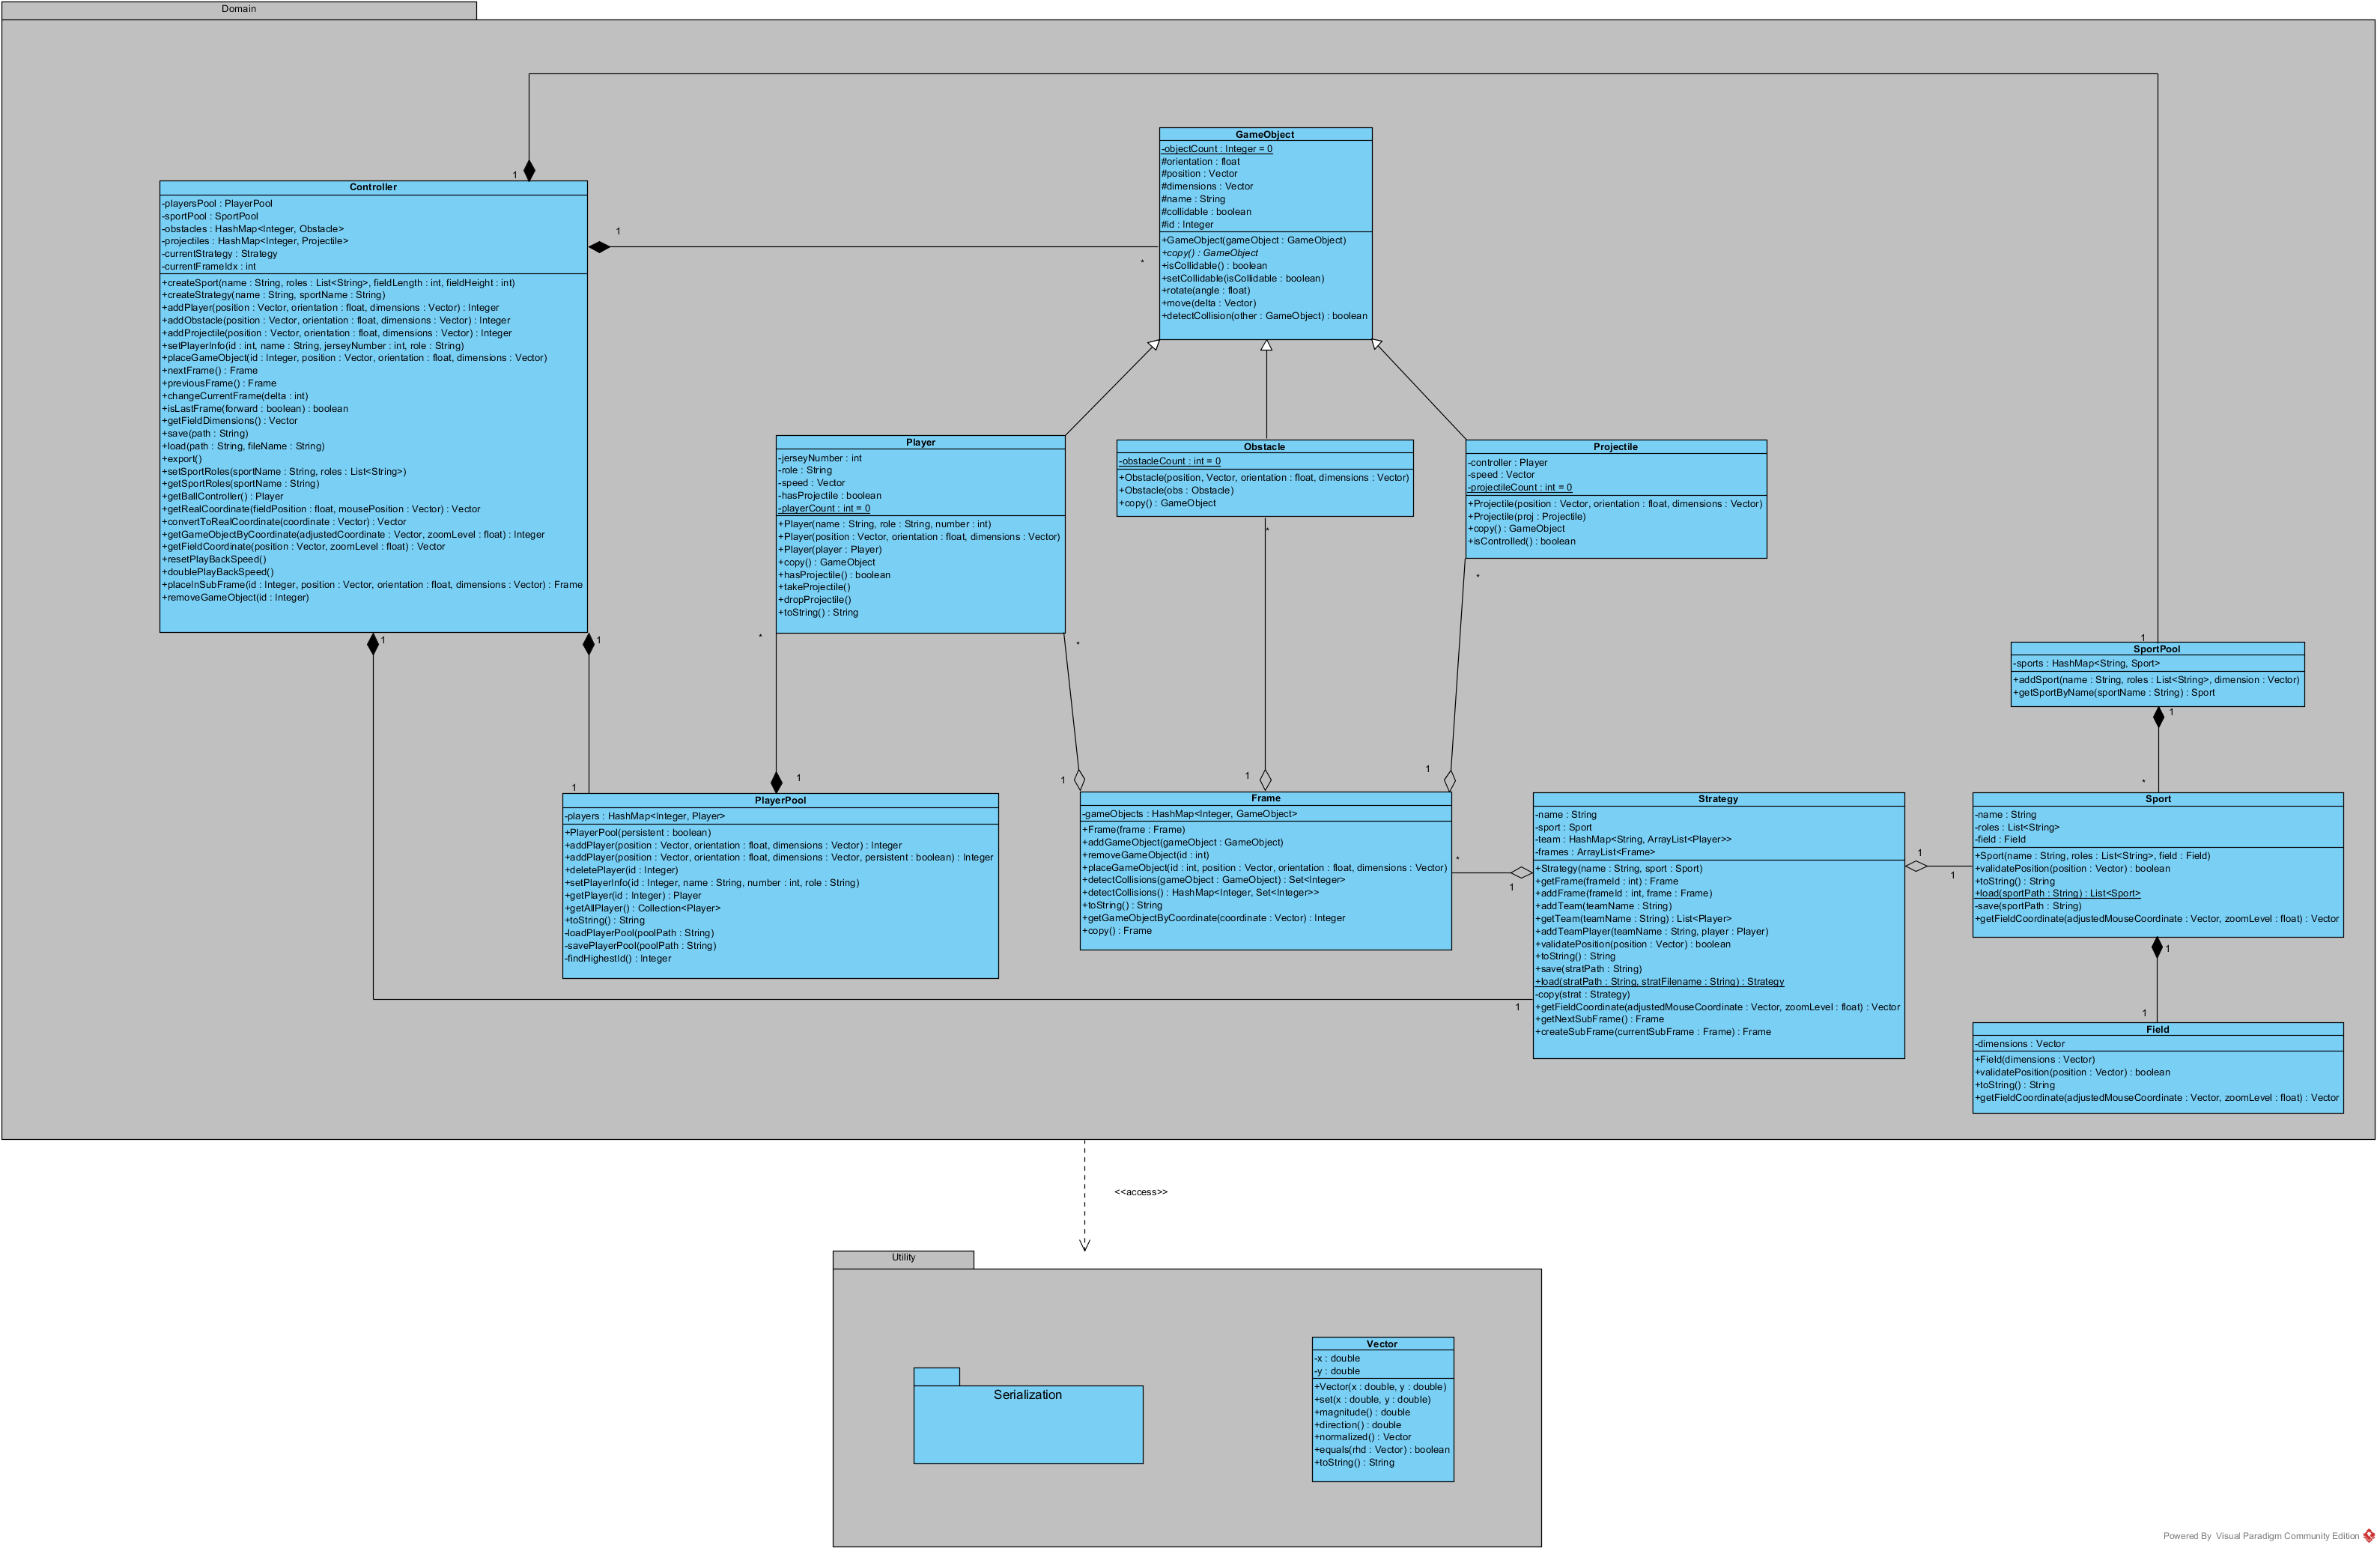
\includegraphics[scale=0.17]{fig/classe_conception_domain.png}
    \caption{Diagramme de classes de conception de la couche domaine}
    \label{fig:domaine_classe}
\end{figure}


\section{Couche présentation}
\label{sec:couche_presentation}

La figure \ref{fig:vue_classes_conception_diag} présente le diagramme de classe de la couche présentation(vue).
La technologie JavaFX est utilisée en union avec le constructeur d'interface graphique \textit{Scene Builder}.
Il y a donc un fichier FXML associé à chacune de ces classes qui contient le code des éléments graphiques.
De prime abord, la classe \textit{RootLayoutController} représente la fenêtre de base de l'application.
Celle-ci contient la barre de menu principal, qui permet d'exécuter la majorité des fonctionnalités du logiciel.
C'est pour cela que ce contrôleur contient une majorité des méthodes permettant la gestion des événements.
Par ailleurs, le patron de conception \textit{Observateur} est utilisé afin de rediriger la gestion de certains événements vers le \textit{RootLayoutController}.
Cela permet d'éviter une duplication du code de gestion des événements tout en maintenant le couplage bas.
Ainsi, la même fonctionnalité peut être exécutée par la barre de menu ou par un bouton dans un autre contrôleur.
Finalement, il est important de comprendre que presque toutes les classes de la vue doivent communiquer avec le contrôleur du domaine. 
Cela n'est pas représenté dans le diagramme, mais il pourrait y avoir une référence au contrôleur dans presque toutes les classes de la vue.


\begin{figure}[htpb]
    \centering
    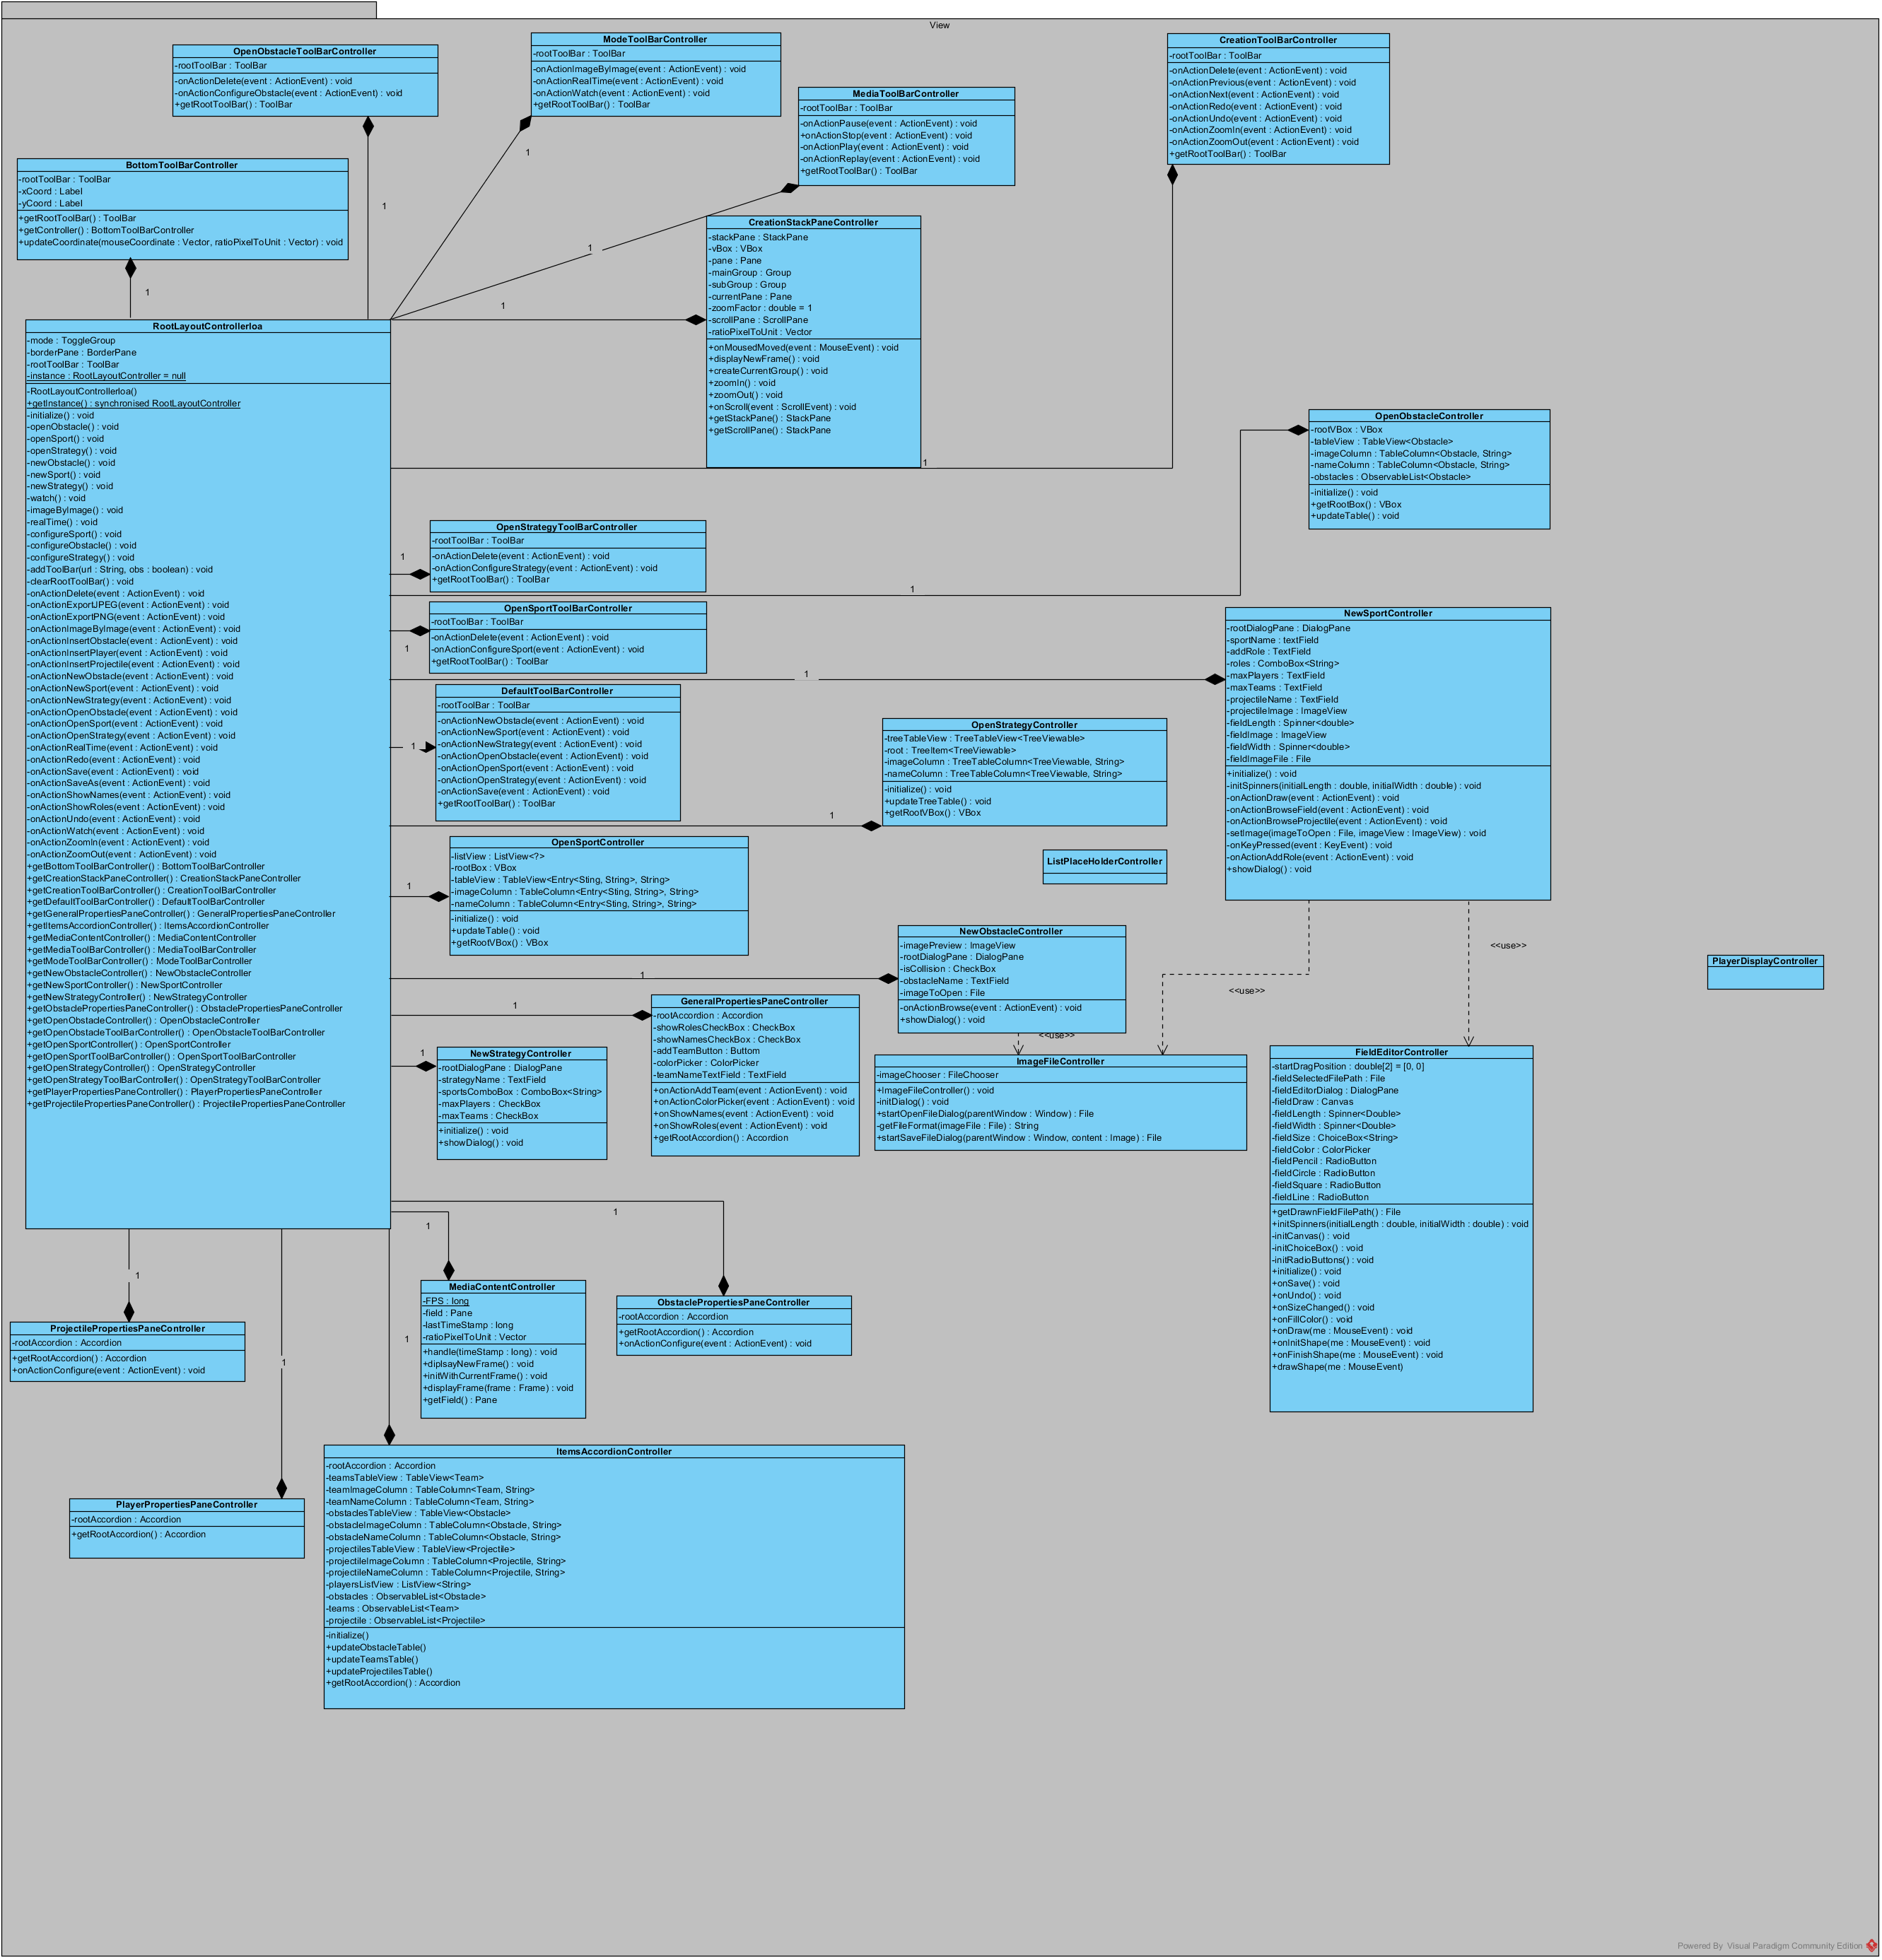
\includegraphics[scale=0.35]{fig/classe_conception_view.png}
    \caption{Diagramme de classes de conception de la couche présentation}
    \label{fig:vue_classes_conception_diag}
\end{figure}

